\documentclass{proposal}
\usepackage{graphicx}
\usepackage[square,numbers]{natbib}
\usepackage{listing}
\usepackage[labelfont=bf]{caption}
\usepackage[outputdir=out]{minted}
\usepackage{chngcntr}
\usepackage[hyphens]{url}
\usepackage{tikz}
\usepackage{hyperref}

\setminted{frame=lines, linenos, autogobble}

\begin{document}

    \counterwithin{listing}{section}


%%%%%%%%%%%%%%%%%%%%%%%%%%%%%%%%%%%%%%%%%%%%%%%%%%%%%%%%%%%%%%%%%%%%%%%%%%%%%%%%%%%%%%%%%%%%%%%%%%%%%%%%%%%%%%%%%%%%%%%%


    \title{ptr-tidy: Automatic refactoring of raw pointers in C++}
    \author{Artem Usov}
    \date{18 December 2020}
    \maketitle
    \tableofcontents
    \newpage


%%%%%%%%%%%%%%%%%%%%%%%%%%%%%%%%%%%%%%%%%%%%%%%%%%%%%%%%%%%%%%%%%%%%%%%%%%%%%%%%%%%%%%%%%%%%%%%%%%%%%%%%%%%%%%%%%%%%%%%%


    \section{Introduction}\label{sec:intro}

    \subsection{Difficulties with Memory Management}\label{subsec:difficulties-with-memory-management}

    % TODO insert info about what memory management/errors are

    Correct memory management is a difficult problem.

    \emph{How difficult one might ask?}

    In a presentation by Matt Miller, a security engineer at Microsoft~\cite{Miller2019}, it is shown that around 70\% of vulnerabilities that are addressed through a security updates are due to memory safety issues.
    In another presentation at the Linux Security Summit~\cite{Gaynor2020} it is shown that in several other top projects such as Firefox, macOS, Ubuntu and Android all had over half of their CVEs attributed to issues with memory safety.
    This is at industry-leading companies who are renowned for hiring top talent.
    Such memory safety vulnerabilities can be exploited, and due to new regulations such as the GDPR, these issues are more commonly exposed to the general public and punished by regulators.
    Such an example is a fine of £20m fine for a British Airways data breach by the British Information Commissioner's Office~\cite{ICO2020}.

    \subsection{Possible Solutions to Memory Management}\label{subsec:possible-solutions-to-memory-management}

    Memory safety errors occur when languages are used that place the tasks of memory management with the programmer, such as C and C++.
    However simply not using these languages is not an option since their inherent danger makes them highly performant, and therefore the only option for a project such as a web browser.

    \emph{What can be done then to address this issue?}

    Engineers at both Microsoft~\cite{Thomas2019} and Mozilla~\cite{Hostfelt2019} converge on Rust~\cite{Balasubramanian2017} as a possible solution.
    Rust is a systems language that offers the same performance as C and C++~\cite{Lin2016}, however its linear type system and memory ownership model also guarantee memory safety.
    The rewriting of a program in a new language is a colossal undertaking, especially in language that has a reputation for being difficult to learn.
    We therefore propose an alternative partial solution to this problem by using a concept from Rust.


%%%%%%%%%%%%%%%%%%%%%%%%%%%%%%%%%%%%%%%%%%%%%%%%%%%%%%%%%%%%%%%%%%%%%%%%%%%%%%%%%%%%%%%%%%%%%%%%%%%%%%%%%%%%%%%%%%%%%%%%


    \section{Statement of Problem}\label{sec:statement-of-problem}

    \subsection{Using Smart Pointers for Memory Management}\label{subsec:using-smart-pointers-for-memory-management}

    Generally pointers are used to give the program access to a resource that cannot be directly included in the program itself, such as a file or a thread.
    However Stroustrup claims that pointers to objects allocated on the free store is dangerous and a \emph{plain old pointer}, or raw pointer as we will refer to them, should not be used to represent ownership~\cite{Stroustrup2018}.

    \begin{listing}
        \inputminted{c++}{code/manual-leak.cpp}
        \caption{Example of memory leaks using manual management.}
        \label{lst:manual-leak}
    \end{listing}

    % TODO insert some information about heap vs stack

    In \autoref{lst:manual-leak} we can see that when using a raw pointer, there are two cases in which the programmer will never free the allocated memory.
    Instead we can \emph{smart pointers}~\cite{Dimov2003} and the concept of \emph{RAII (Resource Acquisition Is Initialisation)} to create resource handles which automatically eliminate resource leaks with no added overhead.
    Firstly there are \emph{unique pointers} which are a pointer that has only a single unique owner at any time.
    We can therefore fix the cases in which we leak the memory using a unique pointer which can be seen in in \autoref{lst:first-example-unique}.
    In the comments, we can see all the locations where \emph{p} exits the scope of the function and where the compiler will insert delete statements, now ensuring that the resource will never get leaked.
    The ownership of a unique pointer can be transferred between variables using \mintinline{c++}{std::move} which moves the ownership from one variable to another.

    \begin{listing}
        \inputminted{c++}{code/first-example-unique.cpp}
        \caption{Example of using a unique pointer to manage memory.}
        \label{lst:first-example-unique}
    \end{listing}

    There also exists a \emph{shared pointer} for resources which may not have a single unique owner.
    Reference counting is used to ensure that after the last owner loses access to the resource, it will finally be freed.
    Shared pointers are suitable to be used in most situations, except in structures which have cyclic references \autoref{subsec:shared-pointer-cycle-analysis}.

    \subsection{Do Smart Pointer Solve Memory Management?}\label{subsec:do-smart-pointer-solve-memory-management?}

    It would appear then that smart pointers could solve most of our memory management issues, however they were only introduced in the C++11 standard.
    The C++ dialects till then did not have any of these language features, with programs being written predominantly in the C++03 standard.
    There remain many such so called \emph{legacy} programs which have not upgraded to newer standards, and even then, it is up to the programmer to properly utilise smart pointers in their code.

    We therefore propose to create an automatic refactoring tool \emph{(ptr-tidy)}, that statically analyses C++ code and aims to refactor usage of raw pointers into smart pointers.
    It will involve a conservative analysis that first and foremost tries to identify raw pointers that only have a single unique owner at any point in the program.
    If this cannot be guaranteed, then a more conservative refactoring to a shared pointer will be applied.

    Given that the language standards are mostly backwards-compatible~\cite{Winters2020}, we can apply these automatic refactoring without changing the runtime behaviour compared to the original programs.

    % TODO reword section title - or move to proposed approach section

    \subsection{The Research Questions}\label{subsec:the-research-questions}

    \emph{"Can the translation of raw pointers into smart pointers using escape analysis be used to make existing C++ code more modern and extendable?"}

    \emph{"Can the tool identify situations in which unique pointers should be used reliably?"}


%%%%%%%%%%%%%%%%%%%%%%%%%%%%%%%%%%%%%%%%%%%%%%%%%%%%%%%%%%%%%%%%%%%%%%%%%%%%%%%%%%%%%%%%%%%%%%%%%%%%%%%%%%%%%%%%%%%%%%%%


    \section{Background Survey}\label{sec:background-survey}

    In this section we will look into the frameworks and algorithms that we will use to enable us to read and refactor C++ code, and secondly identify the locations where we can apply our refactorings.

    \subsection{Clang and LLVM}\label{subsec:clang-and-llvm}

    C++ as a language is massive, and the first capability our tool will need is to be able to parse C++ code.
    Doing this ourselves would be an undertaking that would likely span longer than the time span of the whole project, therefore it was decided early to use an existing parser.
    The most capable and mature C++ parsers will naturally be the parsers used by the most popular compilers.
    This leaves us therefore with a choice between GCC~\footnote{https://gcc.gnu.org/} and Clang~\footnote{https://clang.llvm.org/}.
    The literature~\cite{duffy2014} is fairly clear on the fact that the design of GCC makes it unsuitable for integration with other projects.
    Clang on the other hand allows us access to the Clang abstract syntax tree (AST) and parser internals through consumers and visitors.

    Clang is a front-end to the LLVM framework~\cite{Lattner2004} which transforms C++ code into the LLVM intermediate representation (IR).
    % TODO define SSA
    The LLVM IR is a language-independent, static single assignment (SSA) representation of the program and will be the target on which we apply our analysis to identify refactoring opportunities.
    We believe this choice will lead to several benefits in terms of the analysis power and future usage of the project:
    \begin{itemize}
        \item First, the usage of SSA allows us to efficiently generate a definition-usage graph, therefore allowing an efficient analysis of all the usages of a pointer to identify its number of owners.
        \item Secondly, by separating the parsing and analysis, we make our analysis stage reusable by any other LLVM frontends.
    \end{itemize}

    Clang was also found to be a good choice of library in terms of usability since documentation and examples are readily found.
    The AST that it produces is also rich in information and closely resembles the original code, as can be seen in \autoref{lst:code-to-ast-example}.
    Information such as the line and column numbers are included, which makes programmatically rewriting source code extremely easy.

    \begin{listing}
        \inputminted{c++}{code/code-to-ast.cpp}
        \inputminted[fontsize=\footnotesize]{text}{code/code-to-ast.txt}
        \centerline{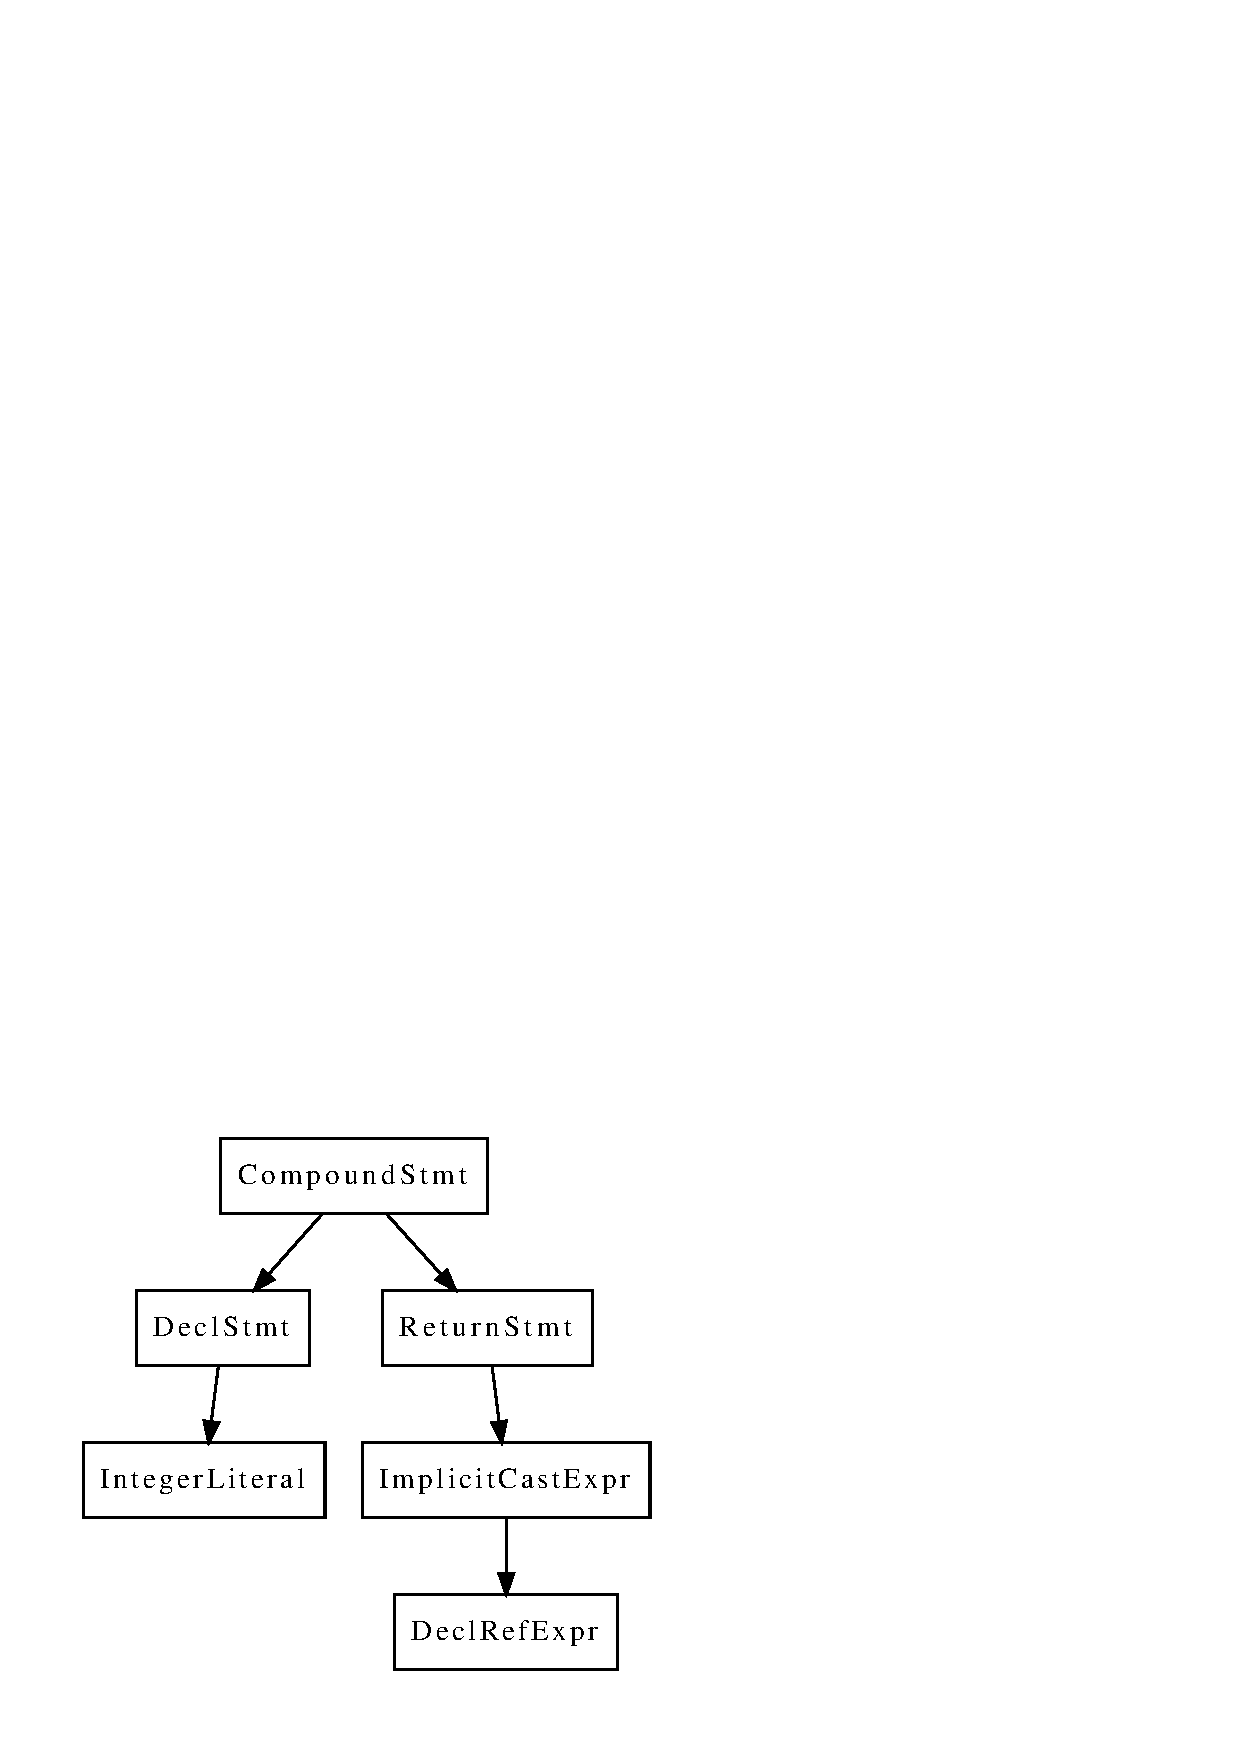
\includegraphics{images/code-to-ast}}
        \caption{Example of converting C++ code to Clang AST. All diagrams show equivalent representation of a small C++ code snippet}
        \label{lst:code-to-ast-example}
    \end{listing}

    \subsection{Pointer Analysis}\label{subsec:pointer-analysis}

    The main capability of the tool is to be able to identify what the maximum number of owners a pointer has at all points of the program execution, for all pointers in any given program.
    If this number for a given raw pointer is one, then we can go about converting all usages of that raw pointer into a unique pointer.
    This will involve changing the type of the initial declaration, its definition as well as removing all deletions of the pointer, which can be seen in \autoref{lst:manual-leak} and \autoref{lst:first-example-unique}.
    If it is more than one then the invariants of a unique pointer cannot be satisfied, and we instead have to use the less performant shared smart pointer.
    A key intuition, mentioned in \autoref{subsec:using-smart-pointers-for-memory-management}, is that a shared pointer can be substituted for most uses of a raw pointer, making it the default fallback.

    A pointer may have more than one owner at a time by copying the pointer to another variable.
    Effectively the address of the underlying region of memory can be accessed through more than one variable, and any accesses of one variable affect the others.
    For example, a pointer may be freed using one variable, and this would invalidate the other variable, causing a memory safety violation if we try to use it.

    We can formalise the notion of copying a pointer by introducing the concept of \emph{escape analysis}.
    Escape analysis is used to determine whether an object \emph{escapes} or is accessible from outside the method or thread that created the object~\cite{Choi1999}.
    It has been used in languages such as Java~\cite{Choi1999} to determine whether an object that is created in a method escapes, and if it does not, meaning it is only used locally in the method, then it can be allocated on the stack rather than the heap as a performance optimisation.
    % TODO pin footnote to specific commit possibly
    Clang also uses escape analysis for a similar kind of optimisation~\footnote{\url{https://github.com/llvm/llvm-project/blob/master/llvm/lib/Analysis/CaptureTracking.cpp}} and also defines the term \emph{pointer capture}.
    A pointer value is captured if the function makes a copy of any part of the pointer that outlives the call.
    We can then see that any pointer that escapes must also be captured since there is no way to refer to an object without being able to determine its address, but not visa versa.
    In \autoref{lst:capture-example} we can see an example where a pointer may be captured but does not escape and in \autoref{lst:escape-example} we see an example of an escaped pointer.

    \begin{listing}
        \inputminted{c++}{code/capture-example.cpp}
        \caption{The pointer is captured in isOdd since the pointer is used for a value that outlives its call, but does not escape since the value of the pointer is not stored anywhere outside the function or thread}
        \label{lst:capture-example}
    \end{listing}

    \begin{listing}
        \inputminted{c++}{code/escape-example.cpp}
        \caption{The pointer is both captured and escapes since the pointer and its value outlive the call of the function and it is accessible by any other method or thread since it is copied to a global variable}
        \label{lst:escape-example}
    \end{listing}

    We can now see that invariant of the unique pointer are only violated in two conditions:
    \begin{itemize}
        \item First, a pointer escapes, as then we do not know where or how the pointer may be used, so we must take a conservative approach and assume the pointer no longer has at most a single unique owner.
        \item Secondly, if a pointer is captured more than once, as we can model a single capture as a move of the unique pointer.
    \end{itemize}

    \subsubsection{Escape Analysis Algorithms}\label{subsubsec:escape-analysis-algorithms}

    Given how we have defined how escape analysis can be used to identify areas of refactoring, we now need to identify a suitable algorithm.

    There has been extensive research on escape analysis for Java, where escape analysis is used to determine whether a object escapes the current method, as then if it can be proven that the object does not escape the method, then it is local to the method invocation and it can be allocated on the stack rather than as a heap variable (the default for all Java objects).

    The escape analysis algorithm described by \citet{Choi1999} is used as the default escape analysis algorithm in the Oracle Java Virtual Machine implementation~\footnote{https://docs.oracle.com/en/java/javase/15/vm/java-hotspot-virtual-machine-performance-enhancements.html} and is widely cited so forms the basis of our investigation.
    Due to how similar C++ and Java are in terms of their Object-Oriented features, will analyse their algorithm as well as the implementations of escape analysis in the LLVM and Go compilers.

    \citet{Choi1999} introduce the abstraction of a \emph{connection graph} (CG) which we will see is also used in other implementations.
    The connection graph captures relationships between heap-allocated objects and object references.
    The graph is used to perform reachability analysis to determine if an is local to a thread or method.
    Most importantly, this abstraction allows for a more powerful interprocedural analysis to be performed.

    The CG is a directed graph $CG = (N_{o} \cup N_{r}, E_{p} \cup E_{d} \cup E_{f})$ where $N_{o}$ is the set of objects.
    $N_{r}$ is the set of reference nodes which include local variables, parameters, fields and global reference variables.
    $E_{p}$ is the set of points-to edges which exists between a reference node which points to object node.
    $E_{d}$ is the set of deferred edges, where a deferred edge from one node $p$ to node $q$ signifies it points to what $q$ points to.
    $E_{f}$ is the set of of all edges between objects that are a field of another object.
    We can see in \autoref{fig:connection-graph-choi} how a connection graph would be constructed for simple Java statements.

    % TODO replace with tikz graphics

    \begin{figure}
        \centering
        \begin{tikzpicture}[scale=0.5]
            \draw (0, 0) circle (1) node{a};
            \draw[->, line width=1pt] (1, 0) -- node[above] {P} (3, 0);
            \draw (3, -1) rectangle node{S1} (5, 1);

            \draw (1, -5) circle (1) node{f};
            \draw (4, -5) circle (1) node{g};
            \draw (7, -5) circle (1) node{h};
            \draw[->, line width=1pt] (4, -1) -- node[above] {F} (1, -4);
            \draw[->, line width=1pt] (4, -1) -- node[above left] {F} (4, -4);
            \draw[->, line width=1pt] (4, -1) -- node[above] {F} (7, -4);

            \node[text width=4.5cm] at (0, 3) {S1: T a = new T(\ldots)};
        \end{tikzpicture}
        \begin{tikzpicture}[scale=0.5]
            \draw (-4, 0) circle (1) node{b};
            \draw[->, line width=1pt, dashed] (-3, 0) -- node[above] {D} (-1, 0);
            \draw (0, 0) circle (1) node{a};
            \draw[->, line width=1pt] (1, 0) -- node[above] {P} (3, 0);
            \draw (3, -1) rectangle node{S1} (5, 1);

            \draw (1, -5) circle (1) node{f};
            \draw (4, -5) circle (1) node{g};
            \draw (7, -5) circle (1) node{h};
            \draw[->, line width=1pt] (4, -1) -- node[above] {F} (1, -4);
            \draw[->, line width=1pt] (4, -1) -- node[above left] {F} (4, -4);
            \draw[->, line width=1pt] (4, -1) -- node[above] {F} (7, -4);

            \node[text width=4.5cm] at (0, 3) {S2: T b = a};
        \end{tikzpicture}
        \caption{A simple connection graph. Boxes indicate object nodes and circles indicate reference nodes (including field reference nodes). Solid edges indicate points-to edge, dashed edges indicate deferred edges, and edges from boxes to circles indicate field edges~\cite{Choi1999}}
        \label{fig:connection-graph-choi}
    \end{figure}

    For each node, we associate an escape set, of either \emph{NoEscape}, \emph{ArgEscape} or \emph{GlobalEscape}.
    \emph{NoEscape} means that the object does not escape the method in which it was created
    \emph{ArgEscape}, with respect to a method, means that the object escapes that method via the method arguments or return value,
    but does not escape the thread in which it is created.
    Finally, \emph{GlobalEscape} means that the object is regarded as escaping globally.
    The initial state for each global node is \emph{GlobalEscape} and \emph{NoEscape} for all other nodes, unless otherwise stated.

    The escape analysis is executed through their defined construction of intraprocedural graphs for each method call.
    We then proceed with the interprocedural by using the CG of the callee to update the CG of the caller.

    At the completion of the escape analysis, all objects which are marked NoEscape and cannot be reached by any node whose state is not \emph{NoEscape} do not escape and are local to the thread in which they are created.
    We show in \autoref{subsec:Interprocedural-analysis} how we can adapt this algorithm to check if the invarients defined in \autoref{subsec:pointer-analysis} are met.

    % TODO move this to the referenced section - Key insight is that we can use defined analysis to check if object escapes. but if each node has at most one object incoming node, it means they are captured at most once

    Go is another language that uses a escape analysis to allocate objects on the stack rather than the heap.
    Their escape analysis algorithms is not defined in the specification of the language, however we can look at the source~\footnote{https://github.com/golang/go/blob/master/src/cmd/compile/internal/gc/escape.go} to determine what algorithm they use.
    Fortunately the comments give a summary of their algorithm, which involves constructing a weighted graph where vertices represent variables, and edges represent assignments between variables.
    They walk the graph, looking for assignment paths that violate the invariants of a variable being allocated on the stack and mark those as requiring heap allocation
    We can see that this approach is highly similar to the use of connection graphs by \citet{Choi1999}, however there is lacking documentation on how they perform interprocedural analysis so their analysis is perhaps weaker.

    Finally, LLVM also uses escape analysis to remove any unnecessary heap allocations.
    The escape analysis algorithm is also not formally defined, however we can also look at the source code~\footnote{https://github.com/llvm/llvm-project/blob/master/llvm/lib/Analysis/CaptureTracking.cpp}.
    We see that the \mintinline{c++}{PointerMayBeCaptured} function uses the fact that the single static assignment (SSA) in the LLVM IR allows for efficient creation of definition-usage chains.
    For any defined value, such as a value initialising a variable, we can traverse all its usages, such as copying to another variable.
    To determine if an object escapes, we analyse all its usages, and all their usages and so on.
    For each usage, we then determine if it is an instruction which would cause the object to escape.
    This leads to a roughly similar analysis as the work by \citet{Choi1999} when considering the intraprocedural analysis alone, as we informally explore a graph of the nodes that represent objects and nodes that obtain references to objects by using the original value in a copy instruction.
    However, its assumption about different instructions are conservative, and it also has no interprocedural analysis, making it the weakest analysis so far.

    \subsection{Memory Safe Languages}\label{subsec:rust}

    There have been many proposed systems languages such as Rust, Swift~\footnote{\url{https://developer.apple.com/swift/}}, D~\footnote{\url{https://dlang.org/}}, Nim~\footnote{\url{https://nim-lang.org/}} or Ada (SPARK)~\footnote{\url{https://adacore.com/}}, however none of these have arguably become mainstream, with Rust and Ada coming closest.

    Swift remains mostly a language for the Apple MacOS and iOS environments for application creation, however it has seen some usage for system programs by companies such as IBM~\footnote{\url{https://github.com/ibm-swift}}.
    Ada or its subset language SPARK are used extensively in certain industries to create verifiable programs for critical systems such as in avionics.
    It is perhaps most well-know for being used in the F-22 fighter aircraft~\cite{malas1997f}, however the use of Ada for those systems show its other weakness in productivity time as it was the cause for several delays in the project, and so it largely remains unused in areas which do not call for such meticulous safety.

    Rust has been the most language in attractive widespread adoption as a systems language.
    Its popularity could be quantified by considering that it is being considered for usage in writing Linux kernel modules~\footnote{\url{https://lore.kernel.org/lkml/CAKwvOdmuYc8rW_H4aQG4DsJzho=F+djd68fp7mzmBp3-wY--Uw@mail.gmail.com/T}}, which cannot be said for C++.
    Following the advice given by many that most systems programs should be written in Rust from now on, we see a potential future usage of our work in the creation of a C++ to Rust transpiler.

    Whilst the automatic refactoring of raw pointers into smart pointers solves some memory issues, the language still offers other ways to invalidate memory safety.
    Equivalent idiomatic Rust would be able to find some of these other errors at compile time.
    A C++ to Rust transpiler would be a much larger undertaking, however we can envision how our project could be helpful.
    Rust affine types~\cite{Balasubramanian2017} are semantically equivalent to C++ unique pointers, in that all values have a single unique owner at any point.
    Therefore our work can identify which pointers are unique and which are not, and those that are not cannot be transpiled into safe Rust, instead requiring to use unsafe blocks to represent such values.

    \subsubsection{Garbage Collected Languages}

    Garbage collected languages encompass some of the most popular programming languages such as Java and Python.
    They are considered to be easier languages than C++ since they remove the need for manual memory management by the programmer.
    In C++, if memory is improperly freed, it gets leaked and can eventually cause out of memory errors.
    Garbage collectors instead run periodically and scan the memory of the program to find objects in memory which were allocated but are no longer used anymore, i.e leaked and then free the leaked objects.
    Languages such as Java~\cite{Tauro2012} use this fully by allocating almost every object on the heap and not freeing any object, instead relying on the garbage collector to clean up.
    They are therefore considered to be easier and more productive to use.

    Garbage collection does also exist for C++ such as the Boehm-Demers-Weiser conservative garbage collector~\cite{boehm2002garbage}.
    So why is garbage collection not used in every language?
    Garbage collection is not zero-cost as the garbage collection algorithm typically stops the execution of the running program to clean up the memory.
    This means that latency or pauses is introduced to every program, and can occur at any point in the execution of the program, such as during the hot path of the program.
    This has led to garbage collected languages being unsuitable for use in systems programs such as OS's, as for example it would be undesirable to have seemingly random latency when interacting with the system.
    There has been research in modern garbage collection algorithms such as ZGC~\cite{ZGC} and Shenandoah~\cite{flood2016shenandoah} for Java which aim to reduce the number and duration of pauses where the garbage collector runs, increasing the responsiveness of the Java virtual machine.
    However, even with much reduced duration of pauses, it may still be unsuitable for some systems with strict latency requirements such as OS's or financial systems.


%%%%%%%%%%%%%%%%%%%%%%%%%%%%%%%%%%%%%%%%%%%%%%%%%%%%%%%%%%%%%%%%%%%%%%%%%%%%%%%%%%%%%%%%%%%%%%%%%%%%%%%%%%%%%%%%%%%%%%%%


    \section{Proposed Approach}\label{sec:proposed-approach}

    State how you propose to solve the software development problem.
    Show that your proposed approach is feasible, but identify any risks.

    \subsection{Shared Pointer Cycle Analysis}\label{subsec:shared-pointer-cycle-analysis}

%%%%%%%%%%%%%%%%%%%%%%%%%%%%%%%%%%%%%%%%%%%%%%%%%%%%%%%%%%%%%%%%%%%%%%%%%%%%%%%%%%%%%%%%%%%%%%%%%%%%%%%%%%%%%%%%%%%%%%%%


    \section{Work Plan}\label{sec:work-plan}

    Show how you plan to organize your work, identifying intermediate deliverables and dates.


%%%%%%%%%%%%%%%%%%%%%%%%%%%%%%%%%%%%%%%%%%%%%%%%%%%%%%%%%%%%%%%%%%%%%%%%%%%%%%%%%%%%%%%%%%%%%%%%%%%%%%%%%%%%%%%%%%%%%%%%


    \bibliographystyle{plainnat}
    \bibliography{proposal}
\end{document}
